\documentclass[12pt, svgnames]{article} %draftclsnofoot 
%for 
%double spacing
\usepackage{amsmath}
\usepackage{amssymb}
\usepackage{fullpage}
\usepackage[round,numbers]{natbib}
\usepackage{multirow}
\usepackage{booktabs}
\usepackage{graphicx}
\usepackage{float}
\usepackage{../ltx/edcomms}
\usepackage{../ltx/setupComments}
\usepackage{hyperref}
\usepackage{geometry}
\usepackage{changepage}
\usepackage{adjustbox}
\usepackage{graphicx}
\usepackage[section]{placeins} % Prevents floats from floating across sections
\usepackage{tabularx}
\usepackage{amsfonts}
\usepackage{glossaries}
\usepackage{multirow} %% Used for Traceability matrix
\usepackage{listings}
\usepackage{calc}
\usepackage[simplified]{pgf-umlcd}
\usepackage[section]{placeins}
\usepackage{enumitem}
\usetikzlibrary{arrows.meta}
\usetikzlibrary{calc}
\usetikzlibrary{positioning}

% ---------------------------
%  Modularized Sections
%---------------------------
\usepackage{subfiles}
\usepackage[noadjust]{cite}
% \input{filename.tex}      %will format input document according to base doc, 
%%can nest
% \include{filename.tex} % cant nest
% \subfile{filename.tex} % used to load child docs
% \usepackage{standalone} %used for importing preamble of child docs
% \usepackage[final]{pdfpages.pdf} %used to insert pdf files; final 
%%format[pages=3-6]
%---------------------------
\let\Oldsubsection\subsection
\renewcommand{\subsection}{\FloatBarrier\Oldsubsection}
\let\Oldsubsubsection\subsubsection
\renewcommand{\subsubsection}{\FloatBarrier\Oldsubsubsection}

\newcounter{acnum}
\newcommand{\actheacnum}{AC\theacnum}
\newcommand{\acref}[1]{AC\ref{#1}}

\newcounter{ucnum}
\newcommand{\uctheucnum}{UC\theucnum}
\newcommand{\uref}[1]{UC\ref{#1}}

\newcounter{mnum}
\newcommand{\mthemnum}{M\themnum}
\newcommand{\mref}[1]{M\ref{#1}}
\makeglossary


% math things
\newcommand{\ra}{$\rightarrow$}



% 
\definecolor{grey}{RGB}{185,185,185}
\definecolor{applegreen}{rgb}{0.55, 0.71, 0.0}
\lstset{ %
  language=Haskell, morekeywords = {family, kind, pattern, expression},
  literate=
  {+}{{$+$}}1
  {/}{{$/$}}1 
  {*}{{$*$}}1 
  {=}{{$=\,\,\,$}}1
  {==}{{$==$}}1 
  %{/=}{{$\not\equiv$}}2
  {==}{{$\equiv$}}2
  {/=}{{$\not\equiv$}}2
  {>}{{$>$}}1 
  {<}{{$<$}}1 
  {\\}{{$\lambda$}}1
  {\\\\}{{\char`\\\char`\\}}1
  {>>}{$>>$}2 
  {:>>=}{{$:>>=$}}2
  %% {>>=}{{\hspace{6pt}\texttt{$>>=$}\hspace{6pt}}}2
  {->}{{$\rightarrow$} }2 
  {>=}{{$\geq$}}2 {<-}{{$\leftarrow$}}2
  {<=}{{$\leq$}}2 {=>}{{$\Rightarrow$} }2
  {|}{{$\mid$}}1 
  {forall}{{$\forall$}}1
  {exists}{{$\exists$}}1 
  {Nat}{{$\mathbb{N}$}}1
  {:\~:}{{$\equiv$}}2
  {\~}{{$\equiv$}}2
  {`In`}{{$\in$}}1
  {.}{{$\circ$\,\,}}1
  ,
  escapeinside={\%*}{*)},
  deletekeywords={>>,>>=,mapM,mapM_,putStrLn,putStr,toInt,show,and,sequence,String,Bool
    ,True,False,Maybe,id,Show,Ordering,Void,Just,Nothing,Int},
  morekeywords={forall, ::, :},
  postbreak={},
  breaklines=true,                
  breakatwhitespace=true,
  %postbreak={  \mbox{\textcolor{grey}{$\rightarrow$}} },
  breakindent = 0pt,
  breakautoindent = true,
  %moredelim=[is][\itshape]{"}{"},
  morestring=[b]",
  mathescape
}

\newcommand{\hstype}[2][0pt]{\attribute{\hspace*{#1}\lstinline[mathescape]|#2|}}

\newcommand{\hstypectr}[1]{\attribute{\hspace*{10pt}\lstinline[mathescape]|#1|}}

\newcommand{\hsfunc}[2][0pt]{\operation{\hspace*{#1}\lstinline[mathescape]|#2|}}

\begin{document}
%\maketitle %% Title page included from Title.tex
\begin{titlepage}
    \begin{center}
        \vspace*{1cm}
        
        \textbf{ Event control action rules for Ampersand}
        
             
        \vspace{1.5cm}
        
        \textbf{Yuriy Toporovskyy (toporoy)\\ Yash Sapra (sapray) \\ Jaeden Guo 
    (guoy34)}
        
        \vfill
        
        Supervised by: Dr. Wolfram Kahl
        
        \vspace{0.8cm}
        
        
\includegraphics[width=0.4\textwidth]{../figures/mac_logo.jpg}
        
        Department of Computing and Software\\
        McMaster University\\
        Ontario, Canada\\
        \today
 
        \vfill 

        The authors herewith license the code which this document accompanies under the GPL v.~3, 
        whose full license text can be found in the source repository. 

    \end{center}
\end{titlepage}

\newpage


\begin{abstract}
%light description
Ampersand Tarski is a tool used to produce functional software documents based 
on business process requirements. At times, logical 
discrepancies arise when system changes occur which violate the 
restrictions set forth by the user. When a system violation occurs, one of two 
things can happen: the change that is meant to take place is adjusted so it no 
longer violates the restrictions or the changes are discarded. The purpose of 
Event condition action rules for Ampersand (EFA) was to replace the exec-engine 
that is currently used to deal with violations; unlike the exec-engine, EFA is 
automated and provides proof of correctness embedded in the code, it able to 
type SQL statements and assure no "dead-ends" occur when queries are executed.
\end{abstract}
\newpage
\tableofcontents
\newpage
\newpage
\section{Introduction}\label{Intro}

This document is a meant as a guide for EFA that includes the motivations taken 
from a business perspective, the mathematical and software foundations that 
resulted in the logical flow of EFA's design, and the testing that took place 
to assure EFA's functionality and correctness.

Currently, Ampersand is readily accessible to the public through Github and it 
is equipped with the ability to assess logical 
discrepancies on sets of data based on user-specified restrictions. Logical 
discrepancies arise when system changes occur which violate the 
restrictions set forth by the user. When a system violation occurs, one of two 
things can happen: the change that is meant to take place is adjusted so it no 
longer violates the restrictions or the changes are discarded. Ampersand is 
used to manipulate data and generate prototypes, although there is a debugger, 
certain errors still slip through. When the system rules are changed by the 
user, all data which are inconsistent with the new system must be eliminated or 
rehabilitated so it can be returned back into the system. Data inconsistencies 
are persistent bugs that can distort the product that Ampersand seeks to 
provide. 

These data inconsistencies are corrected through ECA rules which use process 
algebra (PA) to correct or discard data using violations. EFA is used to 
translate these ECA rules, execute SQL queries to correct violations and 
safeguards the database from illegal transactions.
\subsection*{Ampersand}
\subsection*{Objectives}
\subsection*{Document Guide}

%\section{Business}\label{BusinessSect}
%\documentclass[document.tex]{subfiles}
%\begin{document}

%%{\section{The Purpose of the Project}\label{sec:Purpose}}
\section{Purpose of the project}
\edcomm{YS}{Added the ``AMMBR section'' based on comments from Dr. Kahl. He has verified the section, I'll follow up with a proof read and other section of this document}

Ampersand follows a \emph{rule based} design principle. Rules are integral to an organization
and these are based on some principles and guidelines set by the organization.
Ampersand uses an ECA (Event-Condition-Action\edcomm{WK}{IMO,
  either ``Event-Condition-Action'' or ``Event --- Condition --- Action''}) approach to make sure all rules are satisfied. An ideal information infrastructure supports employees and other stakeholders to maintain the rules of the business. To maintain a rule means to prevent or correct all violations that might occur due to any external or internal factor.
 
 A large portion of the Ampersand system is already in place; the primary focus of this project was to
augment Ampersand with increased capabilities for automation. The module ``Automatically Fix Violations'' in Figure ~\ref{fig:EFAproject} represents the EFA project and where it fits in the current version of Ampersand.
Ampersand relies on the AMMBR \citep{Ampersand} algorithm to help fix these data violations. 
The role 
of AMMBR in Ampersand is to generate functions which can restore violations
in the generated prototype for the given information system. In AMMBR, human involvement is only limited 
to representing rules (in the ADL files). Before our current project was started, there was no way of actually
applying the AMMBR-generated ECA rules to rule-violating database states.
There was therefore also no means to test whether AMMBR is producing
appropriate ECA rules.

The current state of Ampersand uses, as a work-around, the so-called
``Exec engine''. This requires the author of the ADL file 
to write PHP code operating on strings in order to tell Ampersand
how violations should be fixed. This required the author of the 
ADL file to know PHP and have knowledge of the internals of Ampersand,
essentially making information hiding impossible in Ampersand itself if one wanted to use
the ExecEngine. 
 
The EFA project, an extension to the Ampersand system, allows 
the user of Ampersand to generate a prototype for their information
system in which invariants are automatically maintained by code 
generated by EFA, which is derived from the specification given by the user.

The ECA rules, which act as an input to EFA, are translated into human-readable
SQL. This can later be viewed in the command line using the
\verb|``--print-eca-info''| flag.  The generated SQL queries allow the
correctness of AMMBR to be checked by running code generated by AMMBR on actual
databases. Therefore, EFA will be an essential tool for testing AMMBR.

\begin{figure}[!htb]
\begin{center}
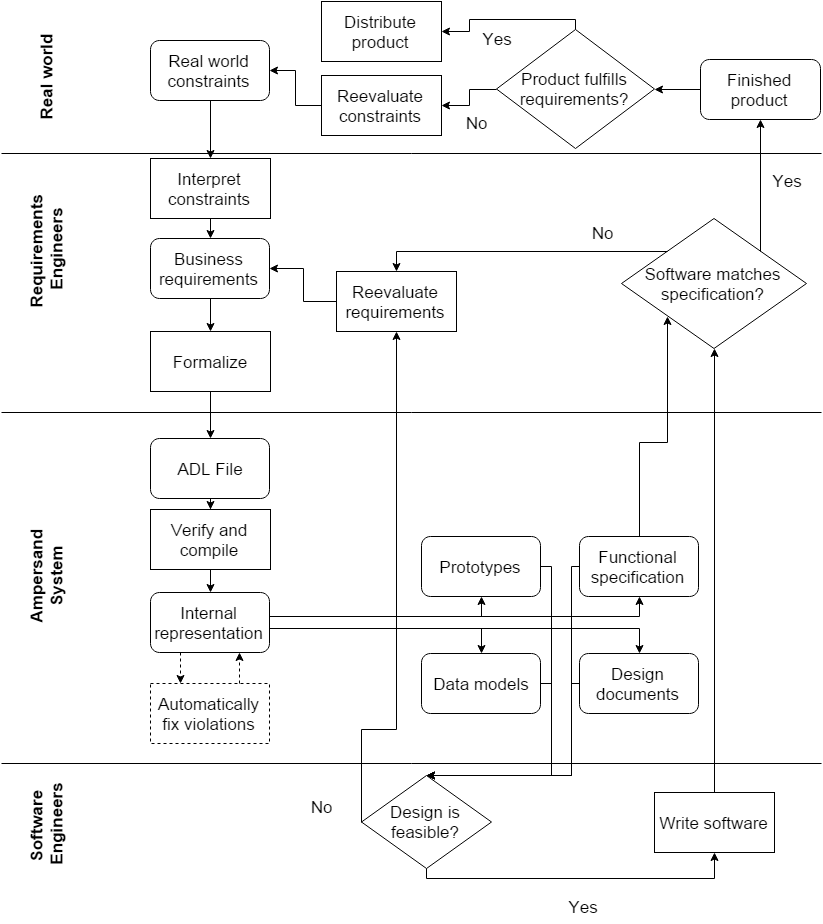
\includegraphics[width=\textwidth]{../figures/business_process}
\caption{Business process diagram representing EFA project represented as a dashed box}~\label{fig:EFAproject}
\end{center}
\end{figure}

\section{The Stakeholders and the intended audience}\label{sec:Stakeholders}
The stake holders of Ampersand are:

\begin{description}
	\item[Ampersand Designers] Responsible for maintaining and developing Ampersand. The overall goal of Ampersand 
is to automate a large part of the software requirements and design process, and EFA fits this goal by greatly increasing
the amount of automation in the system, and therefore decreasing the burden on the user. Furthermore, EFA replaces the ExecEngine,
which allows more of Ampersand to be abstracted and simplifies the maintenance and design of the Ampersand code. 
	\item[The Customer] The requirements engineers using Ampersand to generate prototypes will benefit from the EFA project. 
This will decreases the amount of time 
Ampersand users spend manually inserting PHP code to restore system invariants. The prototypes generated by Ampersand with the 
inclusion of EFA will be less error prone due fewer occurences of violations exposed to the user.
\end{description}

This document is intended to help introduce Ampersand users to EFA 
(ECA rules for Ampersand) -- it provides a basic structure that allows 
individuals to quickly access the information they seek. It is also 
intended to describe the design, implementation, requirements and testing
of EFA for the Ampersand developers. 


\bibliographystyle{alpha}
\bibliography{references}
\end{document}

